\documentclass{article}
\usepackage{amsthm}
\usepackage{amsmath}
\usepackage{amsfonts}
\usepackage{amssymb}
\usepackage{xcolor}
\usepackage[a4paper, top=1.5cm, bottom=1.5cm, left=2cm, right=2cm]{geometry}
\usepackage{graphicx}
\usepackage{tikz}
\usepackage{enumitem}
\graphicspath{ {./images/} }

\newtheorem*{definition}{\color{red}\textbf{Definizione}}
\newtheorem*{theorem}{\color{green}\textbf{Teorema}}
\newtheorem*{oss}{Osservazione}

\newenvironment{example}
{\begin{center}
        \begin{tabular}{|p{0.9\textwidth}|}
            \hline \\ 
            \textit{Esempio}: \\\\ 
        }
        {
            \\\\ \hline
        \end{tabular}
    \end{center}
}
\setlength\parindent{0pt}

\begin{document}
\section{Aritmetica computazionale}
\subsection{Rappresentazione dei numeri reali}
I \textbf{numeri finiti} sono utilizzati dai calcolatori per rappresentare i numeri reali poiché
questi ultimi possono avere un numero infinito di cifre, che i calcolatori, avendo una
memoria limitata, non sono in grado di rappresentare. 

\begin{theorem}[Rappresentazione in base]
    Sia $\alpha$ un numero reale non nullo. Possiamo rappresentare tale numero con una base
    $\beta\geq 2$, un numero intero scelto da noi, nel seguente modo:
    \begin{equation}
        \begin{aligned}
            \alpha&=\pm(\alpha_1\beta^{-1}+\alpha_2\beta^{-2}+\ldots)\beta^p \\ 
            \alpha&=\pm(\sum_{i=1}^{\infty}\alpha_i\beta^{-i})\beta^p
        \end{aligned}
    \end{equation}
    I vari termini dell'uguaglianza vengono detti:
    $$\begin{array}{lll}
        \beta & & \text{base} \\ 
        p & & \text{esponente} \\ 
        \alpha_i & & \text{cifre del numero} \\
        \sum_{i=1}^{\infty}\alpha_i\beta^{-i} & & \text{mantissa}
    \end{array}$$
    Ogni cifra $\alpha_i$ è un numero intero che varia tra 0 e $\beta-1$. Ad esempio, se lavoriamo in base
    10, le cifre saranno numeri interi compresi tra 0 e 9.\\ 
    Per garantire l'unicità della rappresentazione, è necessario che $\alpha_1\neq 0$. 
    Se così non fosse, il numero 13 potrebbe essere rappresentato come 13, 013, 0013, eccetera,
    il che va contro l'unicità della rappresentazione.
\end{theorem}
Possiamo scrivere un numero $\alpha\in\mathbb{R}$ con $\alpha\neq 0$ in due modi:
\begin{enumerate}
    \item \textbf{forma mista}.
        $$\alpha=\begin{cases}
            \pm(0.000\alpha_1\alpha_2\ldots)_\beta & p\leq 0\\
            \pm(\alpha_1\alpha_2\ldots)_\beta & p>0
        \end{cases}$$
    \item \textbf{forma scientifica}. L'idea è quella di spostare il punto decimale al primo numero $\neq 0$ e
        poi moltiplicare il tutto per $\beta^p$ per riportare il numero al suo valore originale.
        $$\alpha=\pm0.\alpha_1\alpha_2\ldots\cdot\beta^p$$
        \begin{example}
            \begin{equation*}
               \begin{aligned}
                   \alpha&=(12.37)_{10} & \alpha&=0.12237\cdot 10^2 \\
                   \alpha&=(0.0045)_{10} & \alpha&=0.45\cdot 10^{-2} \\ 
                         & & &=(4\cdot 10^{-1}+5\cdot 10^{-2})\cdot 10^{-2}
               \end{aligned} 
            \end{equation*}
        \end{example}
\end{enumerate}
\begin{definition}[Numeri finiti]
    L'insieme $\mathbb{F}$ dei numeri finiti è definito come l'insieme dei numeri espressi in base $\beta$
    (dove $\beta\geq 2$), utilizzando $t$ cifre (con $t\geq 1$). Poiché anche l'esponente $p$
    potrebbe essere così grande da non poter essere rappresentato, è necessario limitare
    l'intervallo degli esponenti rappresentabili. Qui, $\lambda$ indica il più piccolo esponente che
    può essere rappresentato e $\omega$ il più grande esponente rappresentabile.
    \begin{equation*}
        \begin{aligned}
            \mathbb{F}(\beta,t,\lambda,\omega)&=\{0\}\cup\{\alpha\in\mathbb{R}:\alpha=\pm0.\alpha_1\alpha_2\ldots\alpha_t\cdot\beta^p, \\
                              &=\{0\}\cup\{\alpha\in\mathbb{R}:\alpha=\pm(\sum_{i=1}^{t}\alpha_i\beta^{-i})\beta^p, \\ 
                              &\text{con } 0\geq\alpha_i<\beta, \text{ per }i=1,2,\ldots,t,\ \alpha_1\neq 0, \lambda\leq p\leq \omega\}
        \end{aligned}
    \end{equation*}
    $\mathbb{F}$ è un sottoinsieme che rappresenta una \underline{discretizzazione} di $\mathbb{R}$. In altre parole,
    $\mathbb{F}$ è un insieme discreto di numeri presi da $\mathbb{R}$, dove ciascun numero può essere espresso al più in $t$
    cifre. Questo significa che gli elementi di $\mathbb{F}$ sono una selezione discreta di numeri reali con una
    precisione limitata a $t$ cifre decimali.
\end{definition}
Per convenzione, utilizzeremo $\alpha$ per scrivere i numeri reali e $\tilde{\alpha}$ per scrivere i numeri finiti.
\begin{example}
    Determinare e posizionare sull'asse reale gli elementi di $\mathbb{F}(2,3,-1,2)$. \\
    I numeri rappresentabili possono essere espressi come:
    $$\tilde\alpha=\pm0.\alpha_1\alpha_2\alpha_3\cdot 2^p$$
    $$\tilde\alpha=\pm(\sum_{i=1}^3\alpha_i\cdot 2^{-i})\cdot 2^p$$
    $\text{con }\tilde\alpha\in \mathbb{F},\ -1\leq p<3 \text{ e }\alpha_1\neq 0$

    L'insieme delle possibili mantisse $m_3$ è dato da:
    $$\begin{aligned}
    m_3 = \{ & 0.100, \\
             & 0.101, \\
             & 0.110, \\
             & 0.111 \} \times \{2^{-1}, 2^{0}, 2^{1}, 2^{2}\}
    \end{aligned}$$
    
    Pertanto, l'insieme degli elementi di $\mathbb{F}(2,3,-1,2)$ è composto da
    33 elementi. Di questi, 16 sono positivi, 16 sono negativi e uno è lo zero.

    Per capire come questi elementi sono posizionati sull'asse reale, li
    portiamo in base 10.
    {
    \renewcommand{\arraystretch}{1.5}
    \[
        \begin{array}{l}
            0.100 = 1\cdot2^{-1}+0\cdot2^{-2}+0\cdot2^{-3}=\frac{1}{2}=\frac{4}{8} \\ 
            0.101 = 1\cdot2^{-1}+0\cdot2^{-2}+1\cdot2^{-3}=\frac{5}{8} \\ 
            0.110 = 1\cdot2^{-1}+1\cdot2^{-2}+0\cdot2^{-3}=\frac{3}{4}=\frac{6}{8} \\ 
            0.111 = 1\cdot2^{-1}+1\cdot2^{-2}+1\cdot2^{-3}=\frac{7}{8} \\ 
        \end{array}
    \]
    \[
        \begin{array}{c|c|c|c}
            \frac{4}{8}\cdot2^{-1}=\frac{4}{16} & \frac{4}{8}\cdot2^{0}=\frac{4}{8} & \frac{4}{8}\cdot2^{1}=\frac{4}{4} & \frac{4}{8}\cdot2^{2}=\frac{4}{2}\\ 
            \frac{5}{8}\cdot2^{-1}=\frac{5}{16} & \frac{5}{8}\cdot2^{0}=\frac{5}{8} & \frac{5}{8}\cdot2^{1}=\frac{5}{4} & \frac{5}{8}\cdot2^{2}=\frac{5}{2}\\ 
            \frac{6}{8}\cdot2^{-1}=\frac{6}{16} & \frac{6}{8}\cdot2^{0}=\frac{6}{8} & \frac{6}{8}\cdot2^{1}=\frac{6}{4} & \frac{6}{8}\cdot2^{2}=\frac{6}{2}\\ 
            \frac{7}{8}\cdot2^{-1}=\frac{7}{16} & \frac{7}{8}\cdot2^{0}=\frac{7}{8} & \frac{7}{8}\cdot2^{1}=\frac{7}{4} & \frac{7}{8}\cdot2^{2}=\frac{7}{2}\\ 
        \end{array}
    \]
    }
    \begin{center}
        \begin{tikzpicture}
            \draw[->] (-2,0) -- (2*5,0) node[right] {R};
    
            % Major ticks with labels
            \foreach \x in {0,1,2,3,4} {
                \draw (2*\x,-0.2) -- (2*\x,0.2) node[above] {\x};
            }
    
            % Minor ticks without labels
            \foreach \x in {0.25, 0.3125, 0.375, 0.4375, 0.5, 0.625, 0.75, 0.875, 1, 1.25, 1.5, 1.75, 2, 2.5, 3, 3.5} {
                 \draw (2*\x,-0.1) -- (2*\x,0.1);
            }
        \end{tikzpicture}
    \end{center}
    Notiamo come questi numeri sono equispaziati tra due potenze consecutive
    della base. Questo ci dà un'idea di come saranno fatti tutti gli insiemi di
    numeri finiti: tendono ad avere una densità maggiore vicino all'origine e si
    diradano man mano che ci si allontana da essa.
    La densità di questi numeri è direttamente influenzata dall'esponente
    negativo. Pertanto, è cruciale trovare un equilibrio tra numeri con
    esponenti sia positivi che negativi.
\end{example}
I numeri finiti sui calcolatori vengono rappresentati seguendo uno standard,
come l'\textbf{ANSI/IEEE 754-1985}, che definisce formati specifici per la
rappresentazione dei numeri in base 2.\\ 
Questo standard definisce 4 formati di numeri finiti, ma solo due di essi sono
rigorosamente specificati. Gli altri due formati sono lasciati alla discrezione
dei produttori di processori.\\ 
Lo scopo di uno standard è garantire la portabilità del codice, così che sia
possibile eseguire lo stesso programma su differenti architetture ottenendo gli
stessi risultati.\\ 
Gli $n$ bit consecutivi dedicati per la memorizzazione di un numero finito
vengono suddivisi tra le $t$ cifre della mantissa ed un certo numero di bit
($\omega-\lambda+1$) per l'esponente $p$, più un bit per il segno del numero.
Alcune tipiche rappresentazioni sono:
\begin{center}
    \begin{tabular} {lll} 
        \textbf{Basic precisione single} & $\mathbb{F}(2,24,-127,128)$ & 32 bit\\ 
        \textbf{Basic precisione double} & $\mathbb{F}(2,53,-1023,1024)$ & 64 bit\\ 
    \end{tabular}
\end{center}
\begin{figure}[!ht]
    \includegraphics[width=0.5\linewidth]{images/IEEE.png}
    \centering
\end{figure}
\newpage
In precisione singola vengono destinati 24 bit alla mantissa (in realtà solo
23\footnote{Essendo sempre $\alpha_1$=1 per la rappresentazione binaria, la
prima cifra può essere sottintesa senza mai essere fisicamente memorizzata.}) e
8 all'esponente ($2^8=256=\omega-\lambda+1,\text{ con }\lambda=-127\text{ e
}\omega=128$), mentre in precisione doppia le cifre della mantissa sono 53
(memorizzati 52 bit) e dell'esponente 11 ($2^{11}=2048=\omega-\lambda+1,\text{
con }\lambda=-1023\text{ e }\omega=1024$).\\ 
Si osservi che l'esponente è memorizzato per traslazione (\textit{exponent
biased}) e che la costante di traslazione (\textit{bias}) è $-\lambda$. Quindi,
se $p$ è l'esponente del numero e $\tilde{p}$ è l'esponente memorizzato,
possiamo trovare l'esponente memorizzato a partire dall'esponente originale
utilizzando la seguente relazione:
$$\tilde{p}=p-\lambda$$
Dato un numero reale non nullo, $\alpha$, per associare un numero finito ad
esso, procediamo come segue:
\begin{enumerate}
    \item \textbf{Rappresentazione esatta}. Se $\alpha$ è scritto nella forma
        $\alpha=\pm(.\alpha_1\alpha_2\ldots)\times\beta^{p}$ tale che
        $\lambda\leq p\leq\omega$, $\alpha_i=0$ per $i> t$, allora è
        rappresentabile \underline{esattamente} come un numero finito $t$ di
        cifre e $\alpha\in \mathbb{F}(\beta,t,\lambda,\omega)$.
    \item \textbf{Rappresentazione approssimata}. Altrimenti 
        $\alpha\notin \mathbb{F}(\beta,t,\lambda,\omega)$ e quindi
        bisogna associargli un numero \underline{approssimato} $\tilde\alpha$
        che indicheremo con $fl(\alpha)$. Si hanno i seguenti casi:
        \begin{itemize}
            \item $p\notin[\lambda,\omega]$, viene segnalata una condizione
                d'errore:
                \begin{center}
                    \begin{tabular}{ll}
                        $p<\lambda$ & \textit{underflow} \\ 
                        $p>\lambda$ & \textit{overflow} \\ 
                   \end{tabular} 
                \end{center}
            \item $p\in[\lambda,\omega]$, ma le cifre $a_i$ con $i>t$ non sono
                tutte nulle, allora viene assegnato un numero finito $fl(\alpha)$
                seguendo due possibili criteri:
                \begin{itemize}
                    \item\textbf{Troncamento} di $\alpha$ alla t-esima cifra
                        $$fl_{T}(\alpha)=\pm(\sum_{i=1}^{t}\alpha_i\beta^{-i})\beta^p$$
                    \item\textbf{Arrotondamento} di $\alpha$ alla t-esima cifra 
                        $$fl_{A}(\alpha)=\pm
                        fl_{T}((\sum_{i=1}^{t+1}\alpha_i\beta^{-i}+\frac{\beta}{2}\beta^{-(t+1)})\beta^p)$$
                \end{itemize}
        \end{itemize}
\end{enumerate}
\begin{example}
    Il numero $\alpha=(0.11011)_2$ ha una mantissa di lunghezza 5, che è più
    lunga delle 3 cifre consentite in $\mathbb{F}(2,3,-1,2)$. Quindi, procediamo
    con l'operazione di arrotondamento:
    \begin{center}
       \begin{tabular}{lll}
           $fl_{A}(\alpha)=$ & $0.11011$ & + \\ 
                        & $0.00010$ & = \\ 
                        \hline
                        & $0.11100$ & \\ 
       \end{tabular} 
    \end{center}
\end{example}
\newpage
\begin{example}
   Consideriamo l'insieme dei numeri finiti $\mathbb{F}(10,5,-50,49)$. Per
   rappresentare un numero finito in questo insieme in memoria, dobbiamo
   definire il numero di posizioni necessarie. Nello specifico:
   \begin{itemize}
       \item\textbf{Segno}: una posizione è riservata per il segno. Se il numero
           è positivo si usa 0; se è negativo, si usa $\beta-1$.
        \item\textbf{Esponente}: due posizioni sono destinate all'esponente.
            Usando la tecnica di memorizzazione per traslazione
            ($p-\lambda=\tilde{p}$), possiamo
            rappresentare gli esponenti da -50 a 49 attraverso valori
            memorizzati da 00 a 99.
        \item\textbf{Mantissa}: cinque posizioni sono dedicate alla mantissa.
   \end{itemize}
   \begin{center}
        \begin{tabular}{ll}
            $\alpha=0.0532=0.532\cdot10^{-1}$ & $fl(\alpha)=04953200$\\ 
            $\alpha=-237141=-0.237141\cdot10^{6}$ & $fl(\alpha)=95623714$
        \end{tabular}
   \end{center}
\end{example}
\begin{oss}
    Siano $x$ ed $y$ due numeri $\in \mathbb{F}$ \underline{consecutivi}
    positivi. Sia $\alpha\in \mathbb{R}$ tale che $x\leq\alpha<y$. 
    \begin{center}
        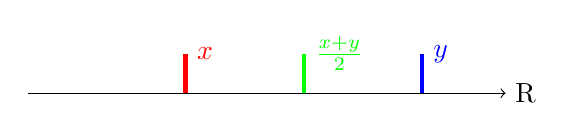
\begin{tikzpicture}
            \draw[->] (0,0) -- (0.5\linewidth,0) node[right] {R};

            \draw[red, ultra thick] (2,0) -- (2,0.5) node[right] {$x$};

            \draw[blue, ultra thick] (5,0) -- (5,0.5) node[right] {$y$};

            \draw[green, ultra thick] (3.5,0) -- (3.5,0.5) node[right] {$\frac{x+y}{2}$};
        \end{tikzpicture}
    \end{center}
    Allora possiamo affermare che $\alpha$ non appartiene all'insieme
    $\mathbb{F}$ perché, per ipotesi, $x$ e $y$ sono consecutivi e non ci può
    essere un altro numero tra loro. Tuttavia, la rappresentazione approssimata
    $fl(\alpha)$ risulta essere:
    \begin{center}
        \begin{tabular}{ll}
            $fl_T(\alpha)=x$ & $fl_A(\alpha)=\begin{cases}
                x & \text{se }\alpha<\frac{x+y}{2} \\ 
                y & \text{se }\alpha\geq \frac{x+y}{2}
            \end{cases}$
       \end{tabular} 
    \end{center}
    L'errore commesso nel troncamento sarà sempre maggiore o uguale dell'errore
    commesso nell'arrotondamento. Questo è il motivo per cui, con una base
    numerica pari, si preferisce utilizzare l'arrotondamento, poiché fornirà una
    migliore approssimazione del numero reale rispetto al troncamento.
\end{oss}
La modalità di arrotondamento dello standard ANSI/IEEE-754 coincide con quella
precedentemente descritta, con la particolarità dell'\textbf{arrotondamento ai
pari}. Questa particolarità si applica quando un numero reale $\alpha$ è esattamente 
equidistante dai numeri finiti consecutivi $x$ ed $y$, in altre parole, 
quando $\alpha=\frac{x+y}{2}$. In questa situazione l'arrotondamento funziona
nel seguente modo:
$$fl_{AP}(\alpha)=\begin{cases}
    x & \text{se }$x$\text{ è pari}\\ 
    $y$ & \text{se }$y$\text{ è pari}
\end{cases}$$
Sempre parlando dello standard ANSI/IEEE-754, per gestire risultati non rappresentabili, 
vengono utilizzati due valori speciali:
\begin{itemize}
    \item \textbf{NaN} 
    \item \textbf{Inf}
\end{itemize}
Invece, di avere un buco vicino allo zero dove i numeri molto piccoli
verrebbero immediatamente arrotondati a zero, vengono inseriti dei numeri ulteriori per
riempire questo buco e permettere ai valori di avvicinarsi progressivamente a zero.
Questo meccanismo è chiamato \textbf{gradual underflow}.\\ 
Per rappresentare questi numeri estremamente piccoli, si fa uso della
rappresentazione \textbf{denormalizzata}. In questa rappresentazione, la
mantissa  non inizia con il solito bit implicito di 1, ma  con una serie di 0.
\subsection{Errori di rappresentazione}
\begin{definition}\leavevmode\
    Consideriamo un valore $\alpha\in \mathbb{R}$. Se $\alpha\notin
    \mathbb{F}(\beta,t,\lambda,\omega)$, allora la sua migliore
    approssimazione all'interno di questo insieme è data da $\tilde\alpha\in
    \mathbb{F}(\beta,t,\lambda,\omega)$. L'approssimazione di $\alpha$ con
    $\tilde\alpha$ introduce un \textbf{errore di rappresentazione}. Per quantificare
    tale errore, definiamo le seguenti metriche:
    {
        \renewcommand{\arraystretch}{1.5}
        \begin{center}
           \begin{tabular}{ll}
                $E_{abs}=\lvert \alpha-fl(\alpha)\rvert$ & errore assoluto \\
                $E_{rel}=\lvert \frac{\alpha-fl(\alpha)}{\alpha}\rvert\text{ se
            }\alpha\neq0$ & errore relativo 
           \end{tabular}
        \end{center}
    }
\end{definition}
Nel calcolo scientifico, l'errore relativo è preferito poiché fornisce una
misura dell'errore ``normalizzata'', che non dipende dalla grandezza dei numeri confrontati.
\begin{example}
    Si eseguano i passi necessari per rappresentare il numero reale
    $(-13.9)_{10}$ in un'area di memoria di 8 bit (1 per il segno, 3 per
    l'exponent biased e 4 per la mantissa), che permettono di memorizzare
    $\mathbb{F}(2,5,-3,4)$ per troncamento e arrotondamento.
    \vskip 0.1in
    \begin{enumerate}
        \item \textbf{Conversione in binario}, prima la parte intera, quindi la parte decimale:
            \begin{itemize}
                \item \textit{Parte intera}:
                    \begin{enumerate}
                        \item Dividi il numero per 2.
                        \item Registra il resto della divisione (sarà 0 o 1).
                        \item Usa il quoziente ottenuto come nuovo numero e
                            ripeti la divisione per 2.
                        \item Continua il processo fino a quando il quoziente
                            diventa 0.
                        \item Leggi i resti della divisione in ordine
                            \underline{inverso}:
                            questo sarà il numero in base 2 della parte
                            intera.
                    \end{enumerate}
                    $$(13)_{10}=(1101)_2$$
                \item \textit{Parte decimale}:
                    \begin{enumerate}
                        \item Moltiplica la parte decimale per 2.
                        \item Registra la parte intera del risultato (sarà 0 o
                            1).
                        \item Usa la parte decimale del risultato come nuovo
                            numero e ripeti la moltiplicazione per 2.
                        \item Continua questo processo finché non ottieni una
                            parte decimale di 0 o si arriva al limite di
                            precisione della mantissa.
                        \item Leggi i numeri interi in ordine di apparizione:
                            questo sarà il numero in base 2 della parte
                            decimale.
                    \end{enumerate}
                    $$0.9\times2=\underline{1}.8$$
                    $$0.8\times2=\underline{1}.6$$
                    $$0.6\times2=\underline{1}.2$$
                    $$0.2\times2=\underline{0}.4$$
                    $$0.4\times2=\underline{0}.8$$
                    $$(0.9)_{10}=(11100\ldots)_2$$
            \end{itemize}
            da cui
            $$(-13.9)_{10}=(-1101.11100\ldots)_2$$
        \item \textbf{Normalizzazione}:
        nello standard IEEE-754, la rappresentazione normalizzata dei numeri
        in virgola mobile prevede che la parte \underline{intera} sia sempre
        1.
            $$(-1101.11100\ldots)_2=(-1.10111100\ldots)_2\times2^{3}$$
        \item \textbf{Calcolo dell'esponente biased}:
            $$p-\lambda=\tilde{p}\rightarrow3-(-3)=6$$
            $$(-1.10111100\ldots)_2\times2^3=(-1.10111100\ldots)_2\times2^{(110)_2}$$
        \item \textbf{Rappresentazione della mantissa}:
            \begin{center}
               \begin{tabular}{cc}
                    arrotondamento & troncamento \\ 
                   1.10111 + 0.00001 = 1.1100 & 1.1011
               \end{tabular} 
            \end{center}
        \item \textbf{Rappresentazione in memoria}: nello standard IEEE-754,
        con una mantissa di 5 bit, solo 4 bit vengono effettivamente memorizzati in memoria.
        \begin{center}
           \begin{tabular}{cc}
               $
               \begin{array}{|c|c|c|c|c|c|c|c|}
                   \hline
                   1 & 1 & 1 & 0 & 1 & 1 & 0 & 0\\
                   \hline
               \end{array} 
               $ 
                &
                $
                \begin{array}{|c|c|c|c|c|c|c|c|}
                    \hline
                    1 & 1 & 1 & 0 & 1 & 0 & 1 & 1 \\
                    \hline
                \end{array}
                $
           \end{tabular} 
        \end{center}
    \end{enumerate}
\end{example}
\begin{example}
    
\end{example}
\end{document}
